\documentclass[../main.tex]{subfiles}
\usepackage{caption}
\begin{document}


\section{Билет 6. Формула Кирхгофа решения задачи Коши для неоднородного волнового уравнения в \texorpdfstring{$\R^3$}{R\textasciicircum 3}. Метод Дюамеля. Принцип Гюйгенса}
% Иваныч техал
\subsection{Формулировка задачи}

\begin{equation} \label{6_1}
    \begin{cases}
        u_{tt} - a^2\Delta u = f(t, x) & t > 0, x \in \R^3 \\
        \while{u}{t=0} = 0 & \\
        \while{u_t}{t=0} = 0
    \end{cases} \;\;\text{ считаем, что } f(t, x) \in C^{0,2}_{t,x}\, \{t \geq 0,\, x \in \R^3\}
\end{equation}

\subsection{Метод Дюамеля}

Сведем задачу к задаче Коши для однородного волнового уравнения. Рассмотрим однопараметрическое семейство задач:
\begin{equation} \label{6_2}
\begin{cases}
    w_{tt}(t, x, \tau) - a^2\Delta_x w(t, x, \tau) = 0 & t > \tau;\ x \in \R^3 \\
    \while{w}{t=\tau} = 0 & \\
    \while{w_t}{t=\tau} = f(\tau, x) &
\end{cases} \;\;\; \tau \geq 0
\end{equation}

Решение задач семейства получаем по формуле Пуассона-Кирхгофа:

\begin{equation*}
    w(t, x, \tau) = \frac{1}{4\pi a^2(t - \tau)}\oiint\limits_{\abs{\xi - x}=a(t-\tau)}f(\tau, \xi)\,dS_\xi \quad \in \; C^{2,2,0}_{t,x,\tau}\,\{t - \tau \geq 0,\, x \in \R^3\}
\end{equation*}

(Под $C^{2,2,0}_{t,x,\tau}$ подразумевается, что $D^\alpha_{t, x}\: w(t, x, \tau)\in C \Forall \alpha\colon |\alpha| \leq 2$)

\begin{statement}
    $$
    u(t, x) = \int_0^t w(t, x, \tau)d\tau \text{ --- классическое решение исходной задачи.}
    $$
\end{statement}
\begin{proof}\hfill
\begin{itemize}
    \item $u(t,x) \in C^2\, \{x \in \R^3,\; t \geq 0\}$
    
    \item $\displaystyle \while{u}{t=0} = 0$
    
    \item Вычислим $\while{u_t}{t=0}$
    
    Интегралы, в которых и пределы, и подынтегральная функция зависят от параметра, дифференциируются по формуле
    $$\pd{}{t} \int_{a(t)}^{b(t)} f(t,x)\,dx = f(t,b(t)) \cdot b' - f(t,a(t)) \cdot a' + \int_{a(t)}^{b(t)} f'_x(t,x)\,dx$$
    В нашем случае $a = 0,\ b = t,\ b' = 1$. Поэтому
    $$\while{u_t}{t=0} = 
    \while{\brs{\underbrace{w(t, x, \tau)|_{\tau = t}}_\text{= 0 из нач. усл. в \eqref{6_2}} + \int_0^t \pd{w}{t}d\tau}}{t=0} = \int_0^0 \pd{w}{t}\, d\tau = 0$$

    \item $\displaystyle \ \Delta_xu = \int_0^t\Delta_x w(t, x, \tau)d\tau$

    \begin{align*}
        u_{tt} &= \pd{}{t}\int_0^t \pd{w}{t}\, d\tau = w_t(t, x, \tau)|_{\tau = t} + \int_0^t w_{tt} (t, x, \tau)\, d\tau
        = f(\tau, x)|_{\tau = t} + a^2 \int_0^t \Delta_x w(t, x, \tau) \, d\tau \\[0.5em]
        &= f(t, x) + a^2\Delta_x u
    \end{align*}
\end{itemize}

Значит, рассматриваемая функция удовлетворяет уравнению.
\end{proof}
Мы доказали следующую теорему:
\begin{theorem}
    Пусть в  задаче \eqref{6_1} функция $f(t,x)$ такова, что $D^\alpha_x\, f \in C\,\{t \geq 0,\; x \in \R^3\}$\\ 
    Тогда функция 
    \begin{equation} \label{6_3}
        u(t, x) = \int\limits_0^t{ \frac{1}{4\pi a^2(t - \tau)}
        \sbrs{\oiint\limits_{\;\abs{\xi - x} = a(t - \tau)}
        f(\tau, \xi)\, dS_\xi} d\tau}
    \end{equation}
    является классическим решением, причем 
    $$
    D^\alpha_{t, x}\, u \in C\,\{t \geq 0, x \in \R^3\}
    $$
\end{theorem}
Суть метода Дюамеля: $f(t, x)$ --- это начальные данные в каждый момент времени.

\subsection{Запаздывающий потенциал}
Преобразуем формулу \eqref{6_3}: 

\begin{align*}
    &\int\limits_0^t \frac{d\tau}{4\pi a^2(t - \tau)}
    \oiint\limits_{\abs{\xi - x} = a(t - \tau)} f(\tau, \xi)\, dS_\xi = 
    \begin{bmatrix} 
        \rho = a(t - \tau) \\
        \tau = t -\rho/a \\
        d\tau = -d\rho/a 
    \end{bmatrix} = 
    -\int\limits_{at}^0 \frac{1}{4\pi a \rho} \frac{d\rho}{a} 
    \oiint\limits_{\abs{\xi - x} = \rho} f \brs{t - \frac{\rho}{a},\; \xi} dS_\xi = \\[1em]
    &= \frac{1}{4\pi a^2} \int\limits_0^{at} d\rho \oiint\limits_{\abs{\xi - x} = \rho} \frac{f(t - \frac{\abs{\xi - x}}{a},\; \xi)}{\abs{\xi - x}}\, dS_\xi
    = \boxed{\frac{1}{4\pi a^2} \iiint\limits_{\abs{\xi - x} < at}\frac{f(t - \frac{\abs{\xi - x}}{a}, \xi)}{\abs{\xi - x}}\;d\xi}
\end{align*}

Выражение в рамке называется \emph{запаздывающим потенциалом}.

\subsection{Общая задача}
$$
\begin{cases}
    u_{tt} - a^2\Delta_x u = f(t, x) \\
    \while{u}{t=0} = u_0(x) \\
    \while{u_t}{t=0} = u_1(x)
\end{cases}
$$

\begin{theorem}[формула Кирхгофа]
    Пусть в общей задаче Коши
    $$
    u_0 \in C^3(\R) \qquad 
    u_1 \in C^2(\R) \qquad 
    f \in C^{0,2}_{t,x}\,\{t \geq 0,\; x \in \R^3\} $$
    Тогда выражение
    \begin{equation*} \label{6_4}
        u(t, x) = \pd{}{t} \frac{1}{4\pi a^2t}\oiint\limits_{\abs{\xi - x}=at}u_0(\xi)\, dS_\xi
        + \frac{1}{4\pi a^2t} \oiint\limits_{\abs{\xi - x}=at}u_1(\xi)\, dS_\xi 
        + \frac{1}{4\pi a^2} \iiint\limits_{\abs{\xi - x} < at} \frac{f(t - \frac{\abs{\xi - x}}{a}, \xi)}{\abs{\xi - x}}\, d\xi
    \end{equation*}

    является классическим решением общей задачи Коши; \; $u(t,x) \in C^2\,\{t \geq 0,\ x \in \R^3\}$
\end{theorem}

\subsection{Принцип Гюйгенса}

Пусть $f=0$, то есть источников нет, а начальное возмущение локализовано в пространстве (носители функций $u_0$ и $u_1$ содержатся в некотором компакте $M$). Тогда в каждой точке воздействие будет локализовано во времени. У такого конечного возмущения есть передний и задний фронты. 
\begin{statement}[Принцип Гюйгенса]
    Возмущение, локализованное в пространстве, приводит к действию, локализованному во времени
\end{statement}

\begin{proof}
Из \hyperref[6_4]{формулы Кирхгофа} видно, что в заданной точке $x_0 \in \R^3$ функция
$u(x_0, t)$ тождественна нулю вне отрезка с концами
$$
t_\text{start} = \frac{1}{a} \cdot \inf_{y\in M}|y-x_0|,
\qquad t_\text{end} = \frac{1}{a} \cdot \sup_{y \in M}|y-x_0|
$$
\end{proof}
\centering
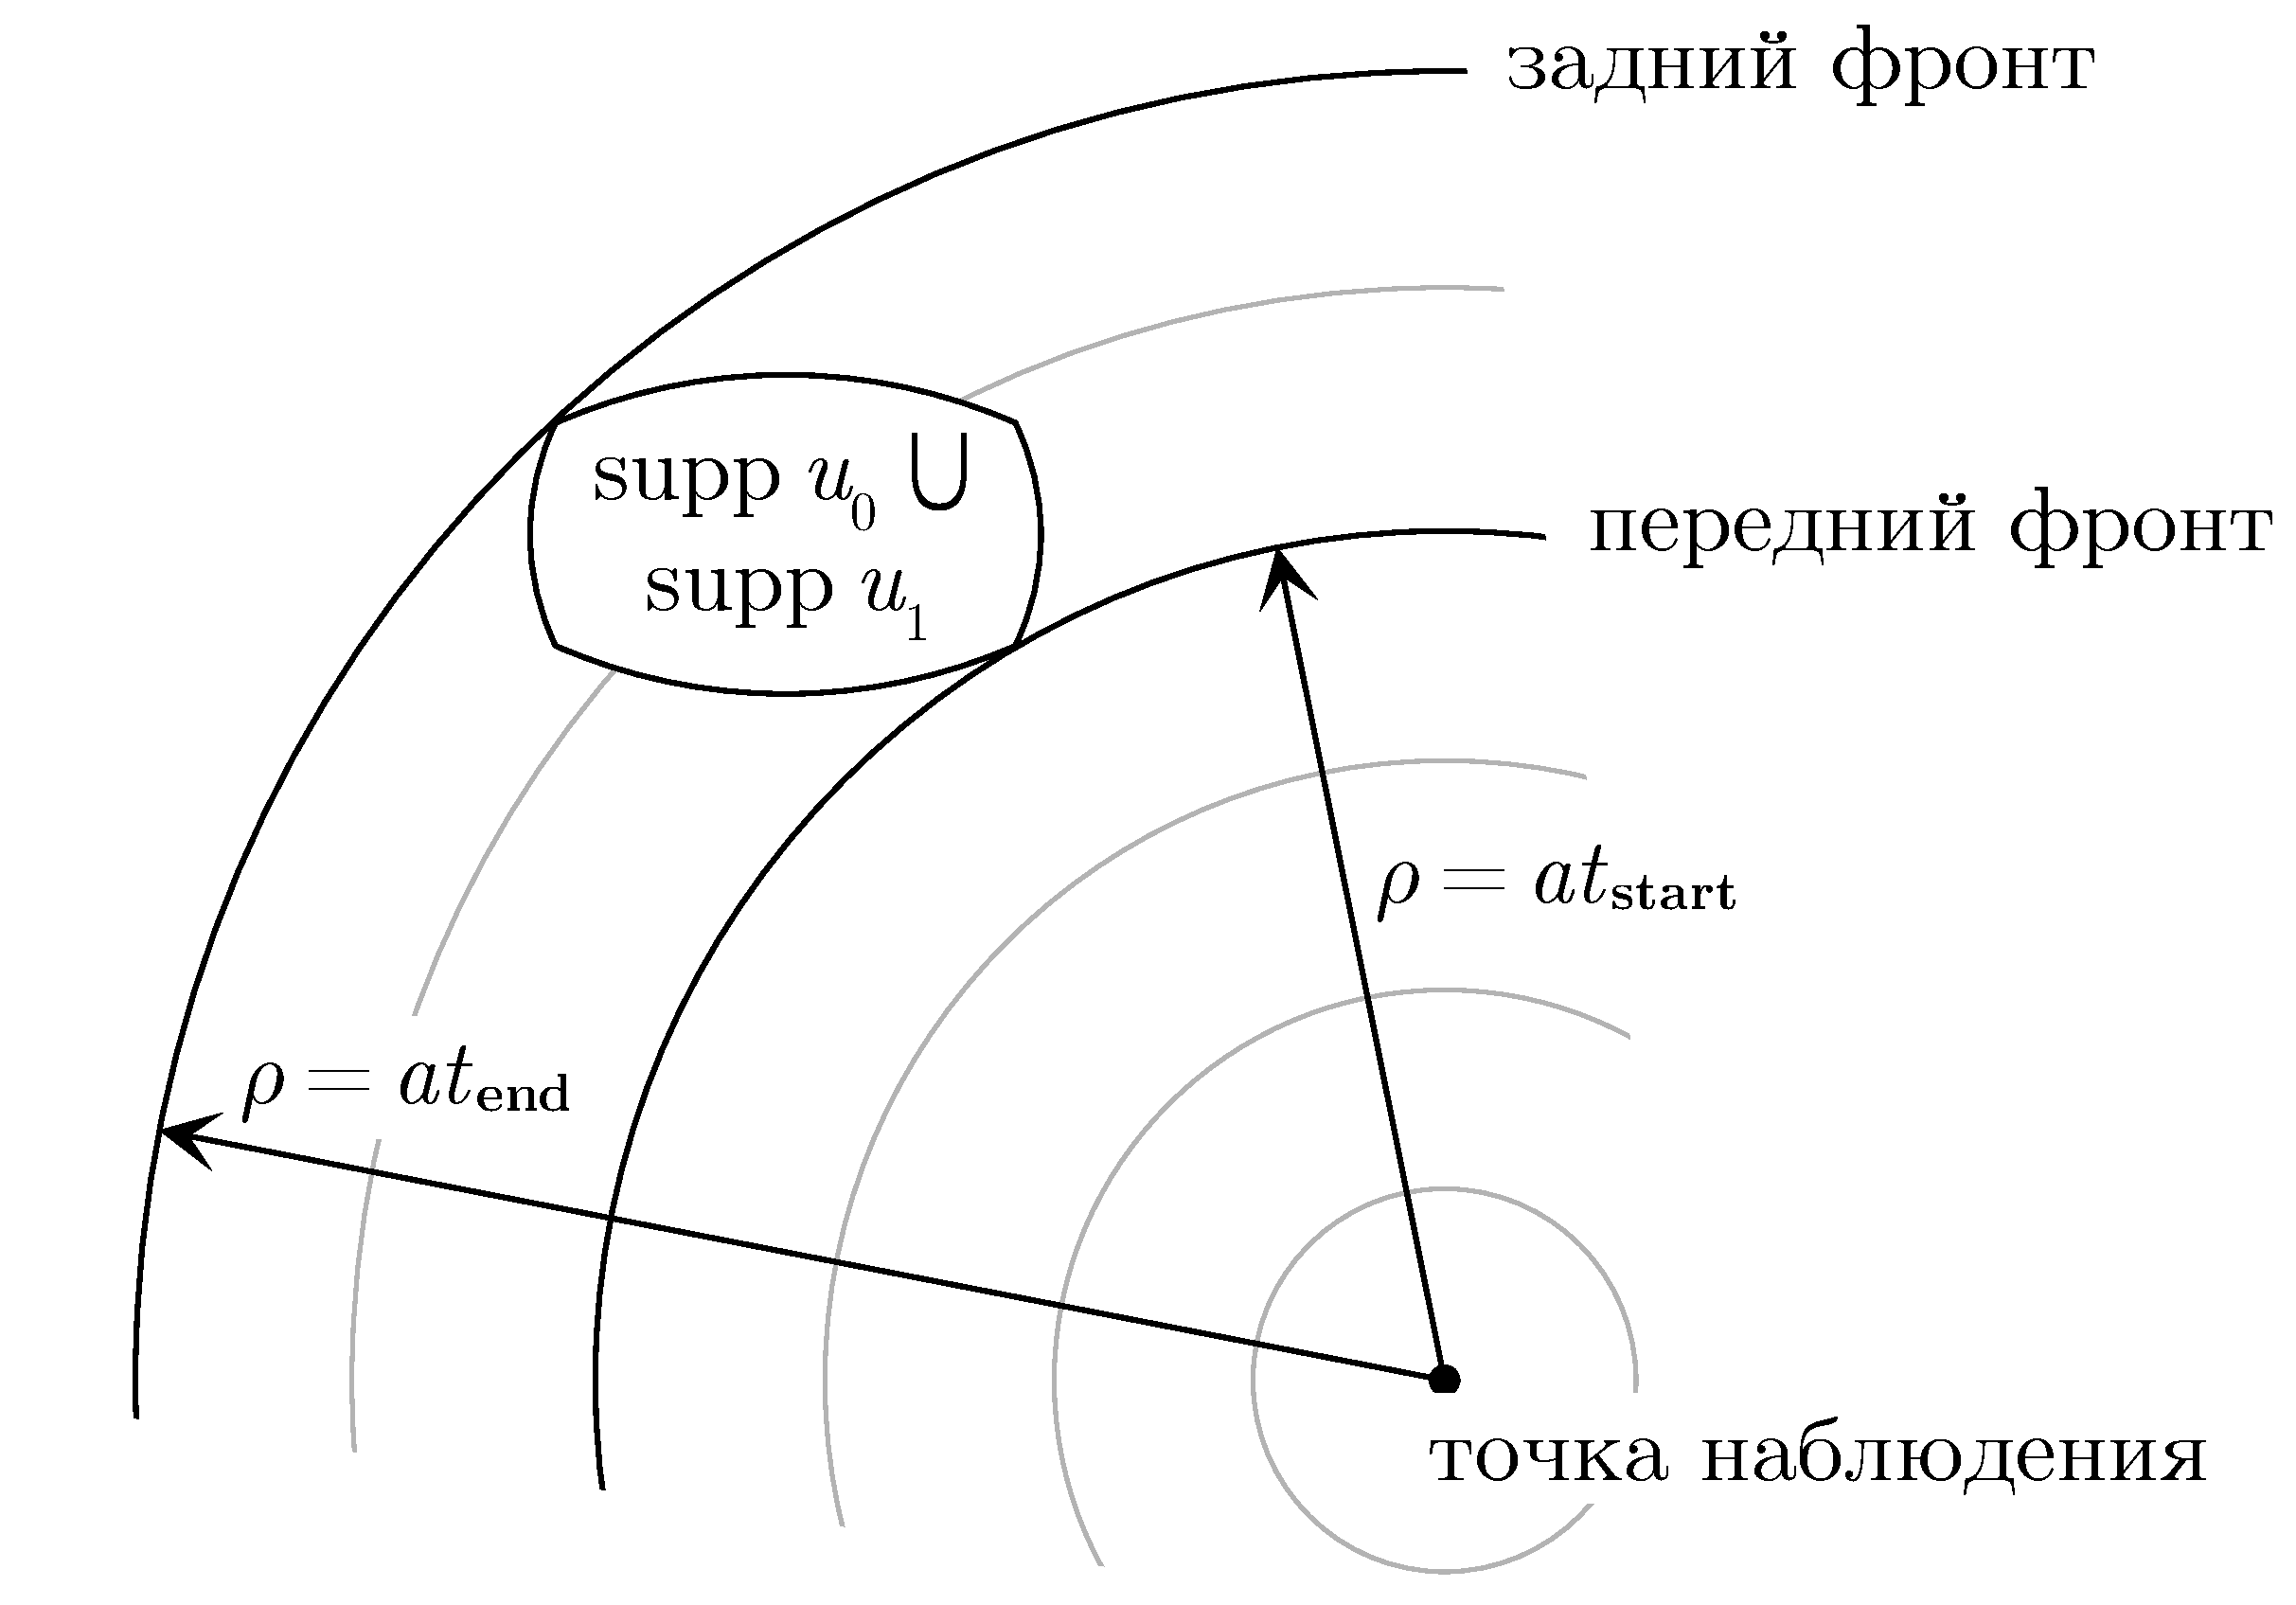
\includegraphics[width=0.45\textwidth]{./pic 6.pdf}

Значение $u(t,x_0)$ равно интегралу по сфере радиусом $|x_0 -\xi| = \rho = at$

\end{document}
